\documentclass[]{article}

\usepackage{enumerate}
\usepackage{scrextend}
\usepackage{amsmath}
\usepackage{graphicx}
\usepackage{fullpage}
\usepackage{float}


\title{Assignment 1 - Medical Image Analysis 2017}
\author{Aslak Niclasen | rql599}




\begin{document}
\maketitle

\section{1D function}
\subsection*{Part 1 - 9}
\textbf{1.} Consider the function
\begin{equation}
	F(x) = x^2 - 70x + 900	
\end{equation}
\\\\which is graphically depicted in the interval from $x \in [1:100]$ in figure \ref{fig:fx} as the blue line.\\\\
\textbf{2.} The minima of the function is located at x = 35, marked in black.\\\\
\textbf{3.} The analytical derivates of $F(x)$ is found to be \hspace{1cm} $F'(x) = 2x - 70$\\\\
\textbf{4. - 5.} You can find the derivatives expressed as a points yellow at figure \ref{fig:fx}. We see as $x$ in $F(x)$ is increasing so is the derivative. Note that not all derivatives of $f(x)$ is shown, but only discrete points [1,2,3...100]. Instead a line would be shown in the general case. It's the minimal value the function can obtain a a specific point in the entire domain of the function. It is characterized as a minima where the function is decreasing towards the point on the left side and increasing on the right side. This property is obtained for all local minima, but here we specifically want the lowest global minima, which is the lowest minima of all minimas of the function.\\\\ 
\textbf{6. - 9.} A discrete version of the function is marked with red dots.\\\\
In order to estimate the resulting value of $F(55.5)$ for the discrete version, we take the resulting change  of $F(55)$ and $F(56)$, average it, and adds it to the first compoment.\\\\
\begin{equation}
	F(55) + \frac{ |F(55) - F(56)| } {2} = 75 + \frac{ | -41 | } {2} = 95.5 
\end{equation}
In order to estime the value of the derivative we look at the rate of change from $F(55)$ to $F(56)$. Since we are evaluating two points, we find the \textit{slope} of the connecting line between the two points.\\\\
\begin{equation}
\frac{y_2 - y_1} {x_2-x_1} = \frac{ F(56) - F(55)} {1} = 116 - 75 = 41
\end{equation}
We now check the error of the discrete findings with respects to the actual function. First we plug in the exact value of 55.5.\\\\
$F(55.5) = 55.5^2 - 70 \cdot 55.5 + 900 = 95.25$\\\\
Next for the derivative at the same point.\\\\
$F'(55.5) = 2 \cdot 55.5 - 70 = 41$\\\\
Thus the respective absolute errors, $E_1$ and $E_2$ are:\\\\
$E_1 = 95.5 - 95.25 = 0.25$\\
$E_2 = 41 - 41 = 0$\\\\

\begin{figure}[H]
\centering
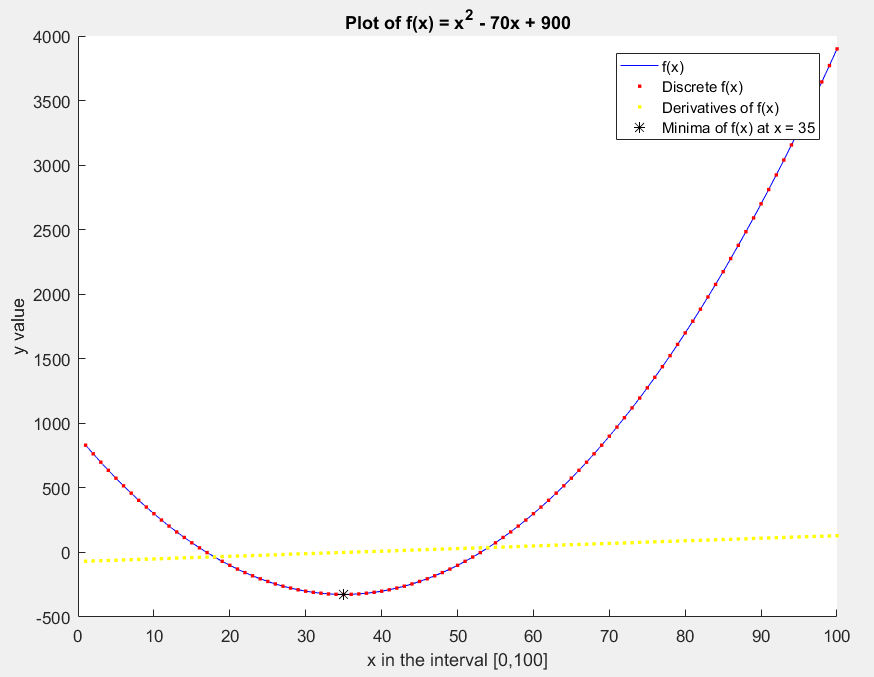
\includegraphics[scale=0.75]{task1.PNG}
\caption{A figure depicting the function $f(x)$ (blue), it's discrete version (red dots), it's derivatives (yellow) and the global minima (black). Note that we only show a subset of the derivatives, depicted as points and not a line here.}
\label{fig:fx}
\end{figure}


\subsection*{Part 10 - 12}
The integral form of a convolution may be expressed as
\begin{equation}
	(f * g)(t) = \int_{-\infty}^{\infty} f(\tau)g(t - \tau) d\tau = \int_{-\infty}^{\infty}	f(t - \tau)g(\tau) d\tau
\end{equation}

And it's derivative can be expressed as
\begin{equation}
	(f * g)'(t) = \int_{-\infty}^{\infty} f(\tau)g'(t - \tau) d\tau = \int_{-\infty}^{\infty}	f'(t - \tau)g(\tau) d\tau 
	= (f' * g) = (f * g')
\end{equation}
The above does however require that we assume the functions $f$ and $g$ are smooth, and integratable over the full domain $(-\infty, \infty)$, which might not always be true.\\\\
Instead of using exhaustive search when finding the minima of the discrete function, one could instead apply gradient decent, or a type of greedy algorithm choosing the better of two points, and then iterate. Both of these are however not prone to errors, if many local minima exists (not in this case) we might get stuck, wheres as exhaustive search always guarentee to find the global minima.

\section{2D function}
\textbf{1.} Consider the function 

\begin{equation} 
	F(x) = x^2 + y^2 - 72x -100y + 3000
\end{equation}
\\\\which is graphically depicted in the interval from $x, y \in [1:100]$ in figure \ref{fig:fxy} as a 3D surface.\\\\

\begin{figure}[H]
\centering
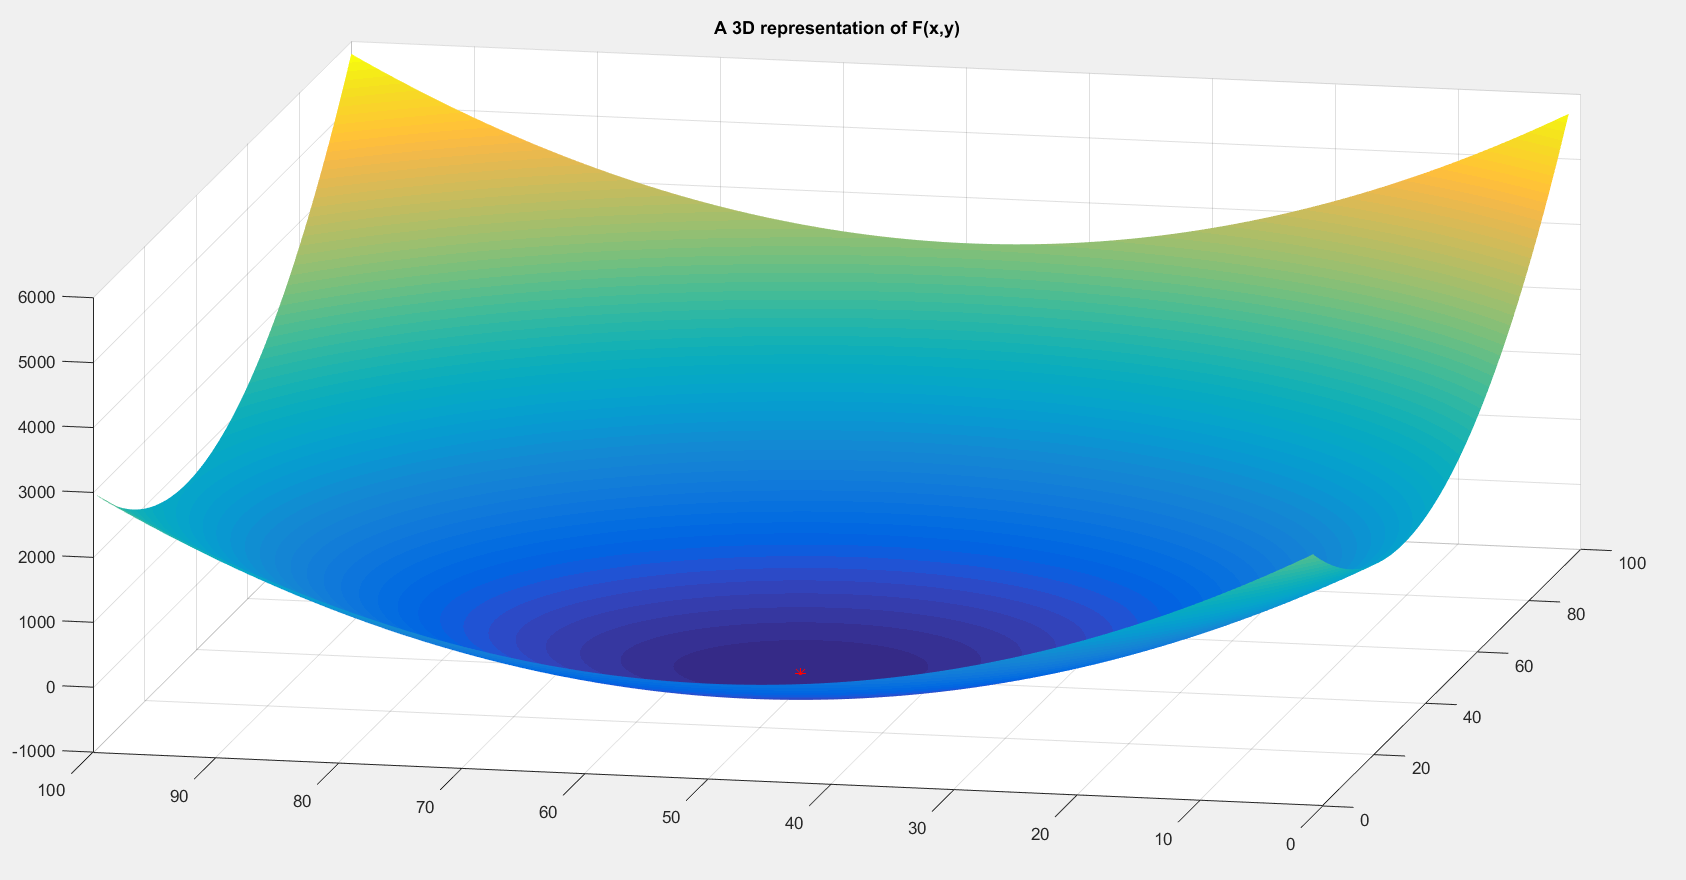
\includegraphics[scale=0.50]{task2a.PNG}
\caption{A 3D surface of the multivarable function $F(x,y)$ in the interval $x,y \in [1:100]$. The global minima is marked with a red * at location (36,50) with value -796}
\label{fig:fxy}
\end{figure}
\textbf{2.} The minima of the function is located at (x,y) = (36,50), marked in black.\\\\
\textbf{3.} The analytical partial derivatives are\\\\
$\frac{\partial f}{\partial x} = 2x - 72$\\\\ 
$\frac{\partial f}{\partial y} = 2y - 100$


\textbf{4.} The minima of a 2D function uses the same argument as in 1D. If all nearby points in the surface have a higher value than the assumed minima, then it's a minima. I might be local, but if we check all local minima we can easily pick the lowest if we can find them all. Below is an image of the function in the interval from [1,100].

\begin{figure}[H]
\centering
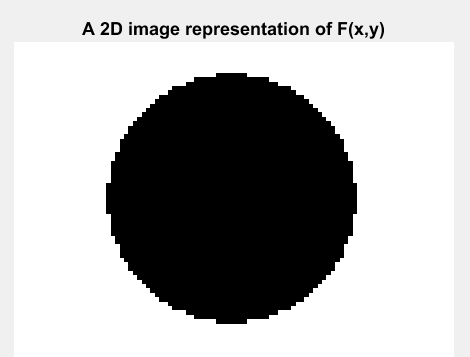
\includegraphics[scale=1]{task2b.PNG}
\caption{An image depicting the function $F(x,y)$ in the interval [1,100].}
\label{fig:img}
\end{figure}

\textbf{5. - 7.}
As previous we compute the average of the change of the values at each individual y value. Then we compute the individual rates of change, and calculate the errors for each. We start with point \textbf{(55.5,55.5)}\\\\
$y = 55 : \qquad F(55) + \frac{ |F(55) - F(56)| } {2} = (-410) + \frac{|-410 - (-399)|}{2} = -415.5$\\\\
$y = 56 : \qquad F(55) + \frac{ |F(55) - F(56)| } {2} = (-371) + \frac{|-371 - (-360)|}{2} = -376.5$\\\\
$ \frac{-410 + (-371)} {2} = -396 $\\\\
The rate of change as previous in a single y position\\\\
$ y = 55 : \qquad \frac{|-410 - (-399)|}{1} = 11 $\\\\
$ y = 56 : \qquad \frac{|-371 - (-360)|}{1} = 11$\\\\
The actual value when evaluated\\\\
$ F(55.5,55.5) = 55.5^2 + 55.5^2 - 72 \cdot 55.5 - 100 \cdot 55.5 + 3000 =  -385.5$\\\\
The rate of change given by the partial derivatives as in 1D\\\\
$ 2x - 72 = 2 \cdot 55.5 - 72  = 40$\\\\
$ 2y - 100 = 2 \cdot 55.5 - 100  = 12$\\\\
The absolute errors are then for the value and the derivtive of it:\\\\
$|-396 - (-385.5)| = \textbf{10.5} $\\\\
$|11 - \frac{40 + 12}{2}| = \textbf{17}$
\vspace{1cm}\\
Do it all again for the point \textbf{(40,40)}\\\\
Average of values\\\\
$ y = 55 : \qquad -670.5$\\\\
$ y = 56 : \qquad -661.5$\\\\
$ \frac{-670.5 + (-661.5)} {2} = -666 $\\\\
The actual value when evaluated\\\\
$ F(40,40) = -680 $\\\\
The rate of change\\\\
$ y = 55 : \qquad 19$\\\\
$ y = 56 : \qquad 19$\\\\
The rate of change given by the partial derivatives\\\\
$2x - 72 = 2 \cdot 40 - 72  = 8 $\\\\
$2y - 100 = 2 \cdot 40 - 100  = |-20|$\\\\
The absolute errors\\\\
$ |-666 - (-680)| = \textbf{14} $\\\\
$ |19 - \frac{8 + 20}{2}| = \textbf{5} $\\\\
I might have swapped the x,y coordinates of the 2D plane when calculating the intermediate discrete values. The error is quite big.

\section{Chapter 1}
\textbf{1.5} The answer is \textbf{d.}: The number of positive observations divided by number of true negative conditions is FPF.\\\\
\textbf{1.6} The last scanner would be the best to pick in my opinion. Even though it missed 0.1 of present obejcts, the other scanner falsely detects 5 times more objects which aren't present. An that propably isn't good, if you want to be reasoanbly sure that the objects you find, are actaully present.\\\\
\textbf{1.7}
Not always. The algorithms for feature detection (maybe blob detection), is applied on an already constructed image. These fundamental yet abstract techniques can be tuned to fit certain problems, but they are not changed in nature. Its' the actual image modality and image construction which is different, not the computer vision algorithms applied after the image is retrieved. However feature detection and image segmentation largely depent on an image internal structure, and may therefore be optimized to medical imaging when desired.\\\\
\textbf{1.8}
Below is 4 images representing an original mammogram, and the same image but with some enhancement teqhniques. A mammogram, depicted with image enhancement teqhniques. Note how LOG mask convolution, applies to much conversion, an only leaves a rough outer border of the breast. Converting this image to grayscale, gives no apparent improvement, but histogram equalization provides some noise but leaves the edges almost intact. So in both these a level of internal breast structure is kept.\\\\
\begin{figure}[H]
\centering
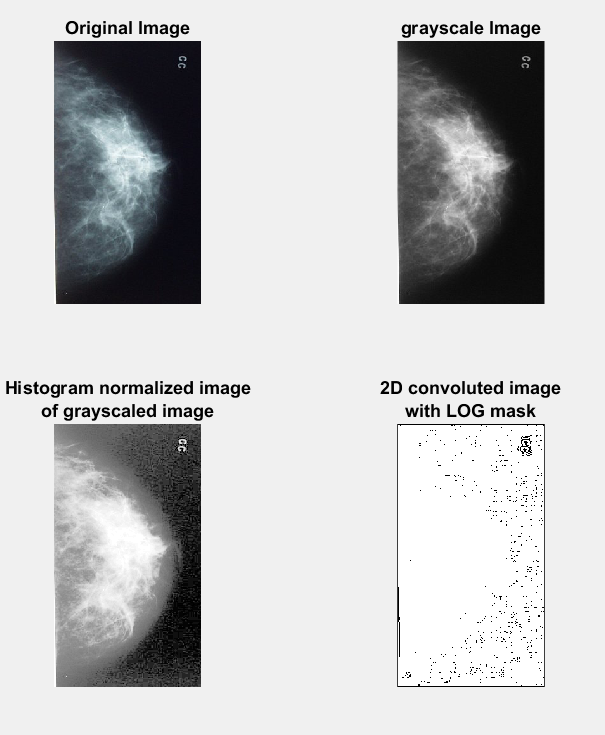
\includegraphics[scale=0.75]{Mammo.PNG}
\caption{A mammogram, depicted with image enhancement teqhniques. Note how LOG mask convolution, applies to much conversion, an only leaves a very rough (if any) outer border of the breast. The internal structure is keept in the other two photos. With histogram equalization we can't really see smaller structures as well as in the original and grayscale image.}
\end{figure}
\textbf{1.9}
Same exercise as 1.8 but with a brain image instead. Note how LOG mask convolution, applies to much conversion, an only leaves a rough border of the brain parts, making them hard to distinguish. The internal structure is somewhat keept in the other two photos. Converting this image to grayscale, gives no apparent improvement, but histogram equalization provides some noise but leaves the edges almost intact.\\\\
\begin{figure}[H]
\centering
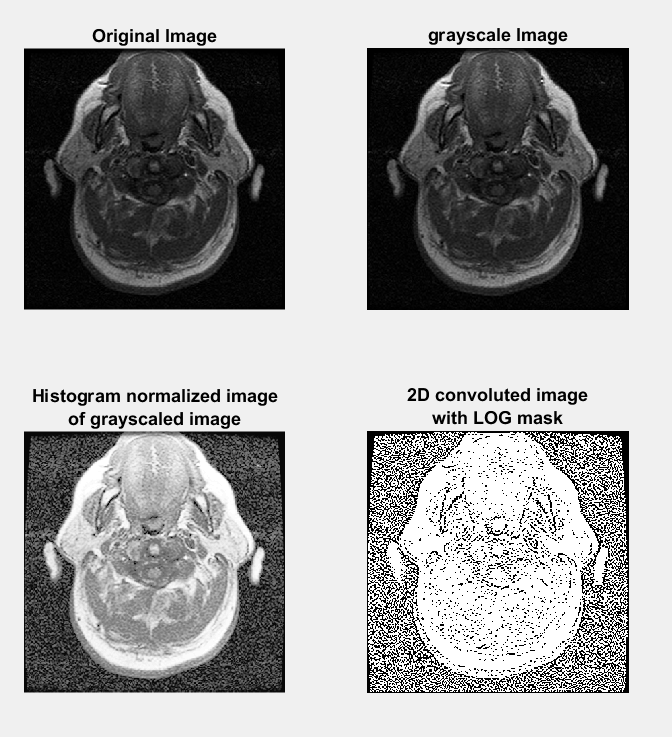
\includegraphics[scale=0.75]{brain.PNG}
\caption{A MRI brain scan, depicted with image enhancement teqhniques. Note how LOG mask convolution, applies to much conversion, an only leaves a rough outline of the brain structures. The internal structure is keept in the other two photos.}
\end{figure}

\newpage
\section{Chapter 2}
\textbf{2.1} A linear system is a system where spatial position is independent, and scalability of a transformation doesn't change the object being modelled. That is, the response of the transformation through the linear system should not change the object itself.\\\\
\textbf{2.6}
Below is shown a binary image of a solid disk, and it's corresponding frequnecy spectrum in the fourier domain. As the images hsow, we can see that both images show how a circular function, is also circular in its fourier domain.
\begin{figure}[H]
\centering
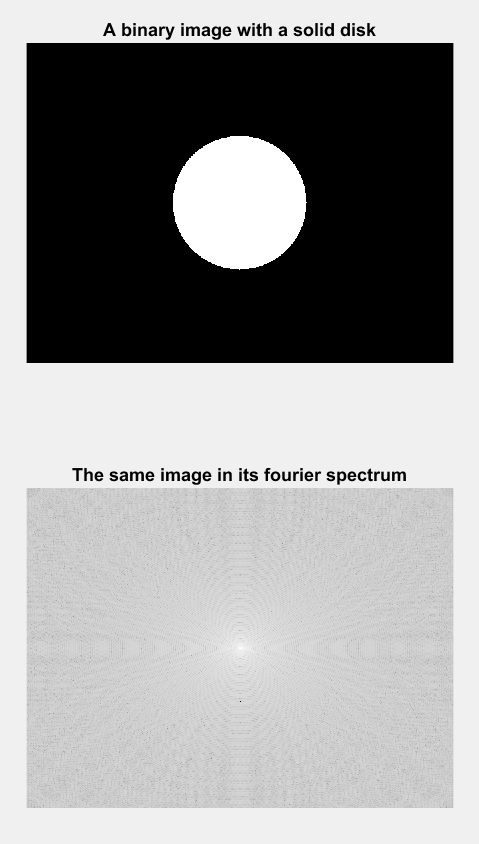
\includegraphics[scale=0.75]{disc.PNG}
\caption{A binary image and its' corresponding frequency spectrum by converting the image to the fourier spectrum}
\end{figure}
\newpage
\vspace{0.5cm}
\textbf{2.13}
Data aquisition is at most 1 KHz. Spatial resolution of object is 1mm x 1mm. Contrast change happens every 0.1ms. We need to see pathology of object at a circular diameter of 1mm.\\\\
First we notice that 1 KHz is equivalent to 1000$s^{-1}$\\\\
Therefore the detector system can detect $\frac{1000s^{-1}}{0.0001s} = 1$ change.\\\\
That is exactly enough to take a single picture before the object changes contrast. Is 1 picture enough, i doubt it, but it might be.\\\\
\textbf{2.14} The following 3 figures (\ref{fig:2Dcam} - \ref{fig:2Drotate}) shows a 2D image which is rotated 30 degrees around the X-axis and 45 degrees around the y-axis. As one can see, i've marked 5 places in the image, and applied the rotation to them as well. The five coordinate pairs marked are\\
\begin{center}
[ (10,10) , (10,244) , (244,10) , (125,125) , (244,244) ]
\end{center}
\vspace{0.5cm}
The rotation matrices used to rotate along the x and y axis' respectively are given by
\begin{equation}
rotate_X =
  \begin{bmatrix}
    1 & 0 & 0 \\
    0 & cos(\theta) & -sin(\theta)\\
  	0 & sin(\theta) & cos(\theta)
  \end{bmatrix}
\end{equation}

\begin{equation}
rotate_Y =
  \begin{bmatrix}
    cos(\theta) & 0 & sin(\theta) \\
    0 & 1 & 0\\
  	-sin(\theta) & 0 & cos(\theta)
  \end{bmatrix}
\end{equation}


\begin{figure}[H]
\centering
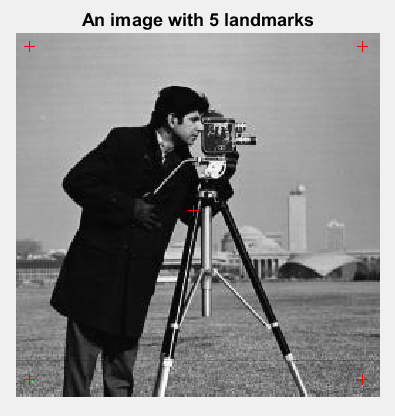
\includegraphics[scale=1]{Image2D.PNG}
\caption{A 2D image with 5 landmarks in red}
\label{fig:2Dcam}
\end{figure}

\begin{figure}[H]
\centering
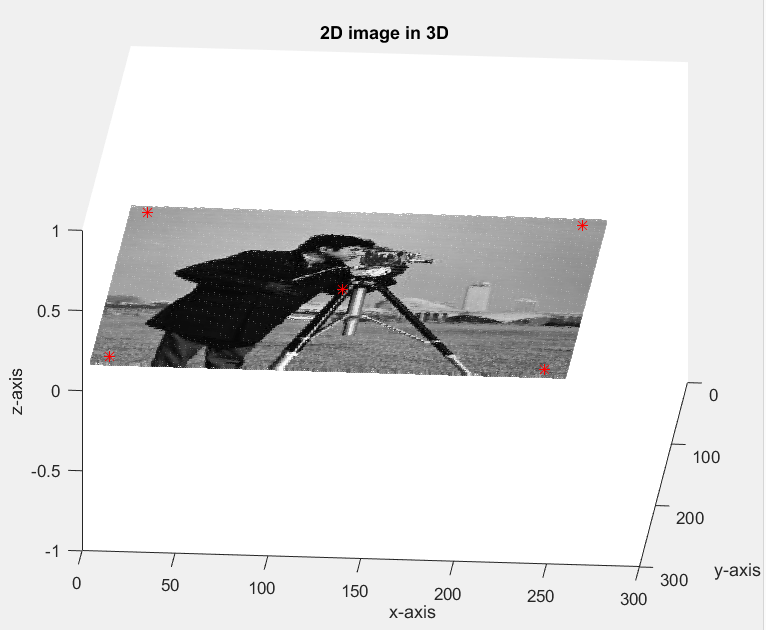
\includegraphics[scale=0.75]{image2D3D.PNG}
\caption{A 2D image with 5 landmarks in red placed in 3D. No transformation is applied}
\label{fig:2D3Dcam}
\end{figure}

\begin{figure}[H]
\centering
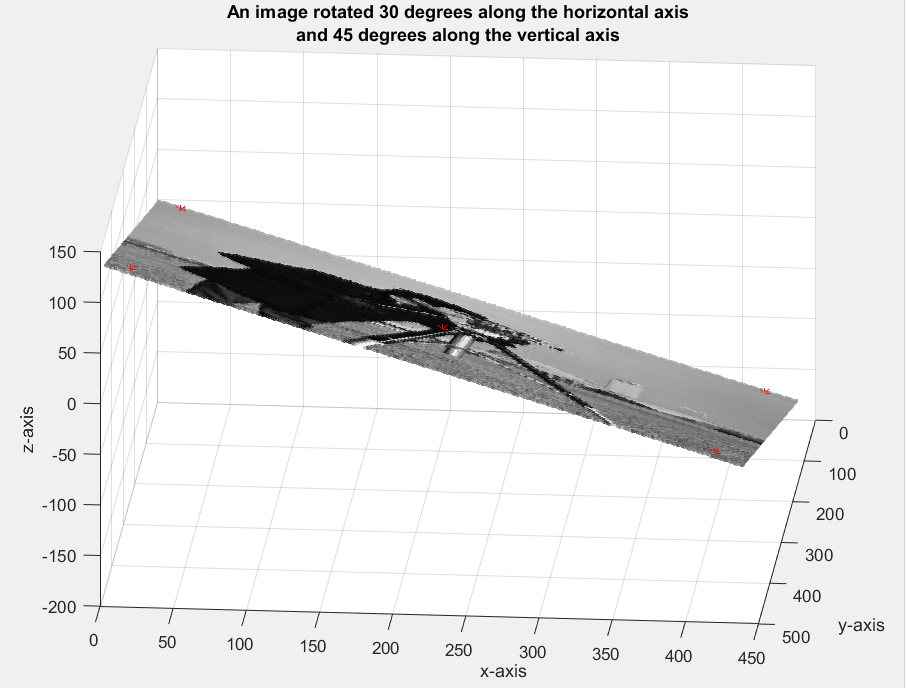
\includegraphics[scale=0.75]{ImgRotated.PNG}
\caption{A 2D image with 5 landmarks in red placed in 3D. A 15 degree rotation along the x-axis and 45 degree rotation along the y-axis have been applied. Note the tilting tilting in 3D as a result of this.}
\label{fig:2Drotate}
\end{figure}

\textbf{2.16}

\section{CT - artificial tommography}
In order to make the artificial tomography i loaded the file, and received a structure containing 76 slices/voxels of 512x512 pixels.
I performed a radon transform (using the build in function \texttt{radon()} in matlab) perpendicular to the z-axis. By doing so, I end up with a 76x729 image projection, based on a specific angle. The image is not 729 always, but is instead padded with zeros at initialization, because the longest distance across the diagonal is 729 pixels in total. For that reason some of the projections are a distinct color at the image edge. However at when showing an image i specify to use the max and min value on a grayscale level of the entire 76x729. For this reason some of the borders become less obvious to spot, due to a similar value in the actual transform. I.e. if the value is close to 0, the border an the value will have almost the same color in the final image shown. The 12 projections obtained form a chest view from around the waist, instead of top down as presented in the original file. The projections are flipped upside down here, but it's easy to see the structure of the lungs (as black) and the ribcage and spine as white in directions where symmetry occurs. As an example, at 90 degrees this picture is clear. It could have been even nicer with more slices in the direction we are currently projecting, becuase they become rather narrow due the the limiting number of voxels.

\begin{figure}[H]
\centering
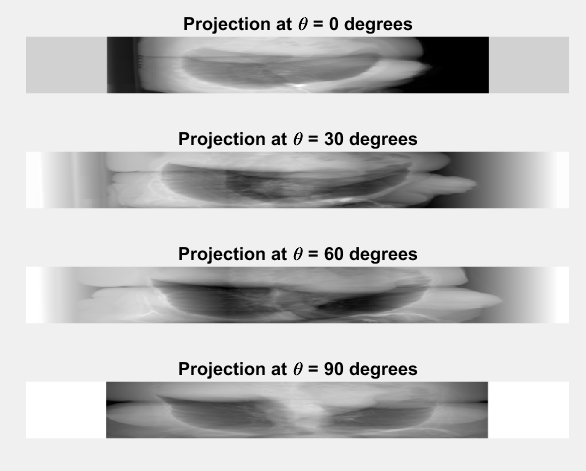
\includegraphics[scale=0.8]{projections1.png}
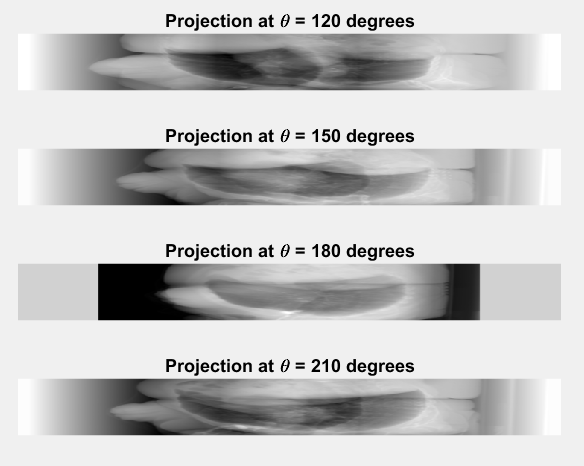
\includegraphics[scale=0.8]{projections2.png}
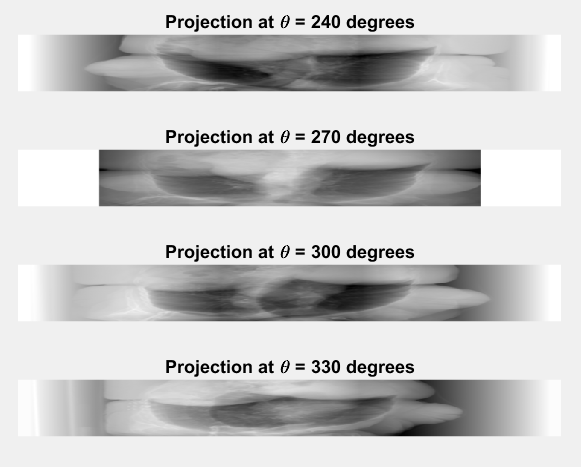
\includegraphics[scale=0.8]{projections3.png}
\caption{All 12 projections at different angles. A stepwise increase of 30 degrees, creates 12 projections in total}
\end{figure}


\newpage
\section{Chapter 4}
\textbf{4.1} The major difference in anatomical and functional imaging is what you want to image in the first place. Where anatomical image modalities focuses on discriminating different constituents, such as bone and tissue, functional image modalities tries to image a function of the body, that is discriminating against different biochemical processes. For anatomical image modalities variations of X-ray exists (radiography, mammography, computed topography), alongside ultrasound MRI. For functional image modalities, MRI, and fMRI, alongside SPECT and PET are excellent modalities.\\\\
\textbf{4.2} X-ray CT is a technique for vizualizing an object. The object is hit with X-ray photons from multiple angles which passes through the object or are scattered. This absortion is called the attinuation and is detected by special detectors. Using algorithms such as backprojection, one can reconstruct the object as an image.\\\\
\textbf{4.3} X rays are generated as the result of interactions of high-speed electrons and heavy atoms. The electron losses energy upon impact and X-rays are scattered in varoius directions\\
In an X-ray generation tube electrons are released by the source cathode
and are accelerated toward the target anode in a vacuum under the potential difference ranging from 20,000 to 150,000 V.\\\\
In the electromagnetic spectrum, X-rays have a wavelength between 10nm - 0.001nm. There are soft X-rays (10nm - 0.1nm) and har X-rays (0.1nm - 0.001nm) The choice of using X-rays as a mean in image modalities is because the have high energy. This makes it easier for the rays to penetrate objects we wish to model. The specific range for medical applications lies within (0.1nm - 0.01nm) because the attenuation can distinguish bones, soft tissue and air in medical diagnostics procedures. Furthermore the short wavelength gives us high resolution images within submillimeter accuracy. If one uses X-rays for therapeutic procedures it's usually higher than in diagnostics purposes, because the photon energy is much higher - an thus in diagnostics purposes we would get less attenuation effect.\\\\
\textbf{4.4} Basically there are two major types of detectors. Ionization detectors, and solid state detectors. Ionization detectors are used in X-ray CT, while solid state detectors are used in digital radiography and mammography.\\\\
\textbf{4.5} X-ray mammography is difficult because breast tissue is hard to attinuate. Thus higher resolution is required to detect early stages of breast cancer, but in order to minimize exposure to the breast, high sensitivity must also be taken into account, to minimize scattering of radiation. This is a tradeoff between high resolution and cancer risk. Newer methods uses special X-ray tubes, brest compression devices antiscatter grids and other approaches.\\\\
\textbf{4.6} As mentioned in 4.4 it's a solid state detector. It usually uses a phosphor screen or scintillation material thallium-doped CsI layer optically coupled with CCDs (Charge coupled devices).\\\\
\textbf{4.7} Iodine based contrast agents are used in X-ray imaging. They help enhance visibility of arteries and blood vessels particular.\\\\
\textbf{4.8} The second-generation X-ray CT scanners used a fan-beam geometry with a divergent X-ray source and a linear array of detectors.\\
The fourth-generation X-ray CT scanners use a detector ring around
the object. The X-ray source provides a divergent fan beam of radiation to cover the object for a single ring of detectors. Scanners with multiple
rings of detectors utilize a cone beam to cover multiple slices (8 – 12) . Recent fast spiral CT scanners use a spiral movement instead of parallel movement for selection of axial slices.\\
The fourth-generation X-ray CT scanners normally use a ring of 720 or more detectors that are equally spaced around the circumference of a circle. The detectors used here are ionization chambers filled with xenon gas or scintillators with photomultiplier tubes.\\\\
\textbf{4.9} As mentioned above the forth-generation scans in a parallel movement while a spiral CT scans in a spiralling movement. In a spiral CT scanner the object is moved in the scanner, while it's stationary in the fourth generation. The spiral CT scanner requires better detectors because the datacollection is continuous.\\\\
\textbf{4.10} If the pitch is changed from 1 to 2, the movement  if a slice is the same size is doubled. This means that there is no effect on the radiation dose, unless rapid movement creates a problem. I would assume this isn't the case, and therefore the radiation dose isn't affected by the pitch.\\\\
\textbf{4.11} We want to calculate the number of light photons emitted from a single X-ray photon with a total energy of 25 keV. Since we know the Total energy and the wavelength we can apply the following formular:

\begin{equation}
	E = \frac{hc}{\lambda}
\end{equation}
Where c, and h are constants, the speed of light and Planck's constant. E is the total energy and $\lambda$ is the wavelength. First lets convert 25 keV to Joule\\\\
25 keV $= 4.00544 \cdot 10^{-15}$J\\\\
Next we insert the wavelength into the formluar and find the energy of a single light photon\\\\
$E = \frac{(6.62 \cdot 10^{-3}m^2\frac{kg}{s} (2.99 \cdot 10^8m/s ) )}{425 \cdot 10^{-9}m} = 4.65736 \cdot 10^{-19}$J\\\\
Now that we have the total energy and the energy of a single photon, lets find the number of photons using these two numbers\\\\
$ n = \frac{4.00544 \cdot 10^{-15}J}{4.65736 \cdot 10^{-19}J} \approx 8600$
Thus at only 20\% efficiency the total number of light photons from a single X-ray photon hitting the intensifying screen is\\\\
$8600 \cdot 0.2 = \textbf{1720}$ light photons\\\\
\textbf{4.12} Similar to question 4.7, a contrast agent is an iodine based substance. They help enhance visibility of arteries and blood vessels particular in imaging. A contrast agent is injected into the object directly.\\\\
\textbf{4.13} In order to lower the error by improving the signal to noise ratio (SNR), several options exists. It depends on the X-ray
exposure, source and detector instrumentation, thickness and heterogeneityof the object, scattering, and contrast agents. The SNR of X-ray imaging is proportional to the square root of the product of the exposure time and X-ray tube current.\\ Thus an improvement in SNR can be achieved in a non-harmful manner such as better detectors. Or one could instead expose the object more, which is more dangerous / harmful.


\section{Chapter 5}
\textbf{5.2} Given an external magnetic field of 1.5T the corresponding Larmor frequency of a given nuclei, can be calculated using Larmors equation\footnote{http://mriquestions.com/who-was-larmor.html}.
\begin{equation}
	f_0 = \gamma B_0
\end{equation}
Where $f_0$ is the frequency, $\gamma$ is the gyromagnetic ratio (which is different for each nuclei and can be looked up) in MHz/T, and $B_0$ is the strength of the external magnetic field in Tesla. The 3 different Larmor frequencies for 3 differnet Nuclei is then\\\\
\begin{equation}
	^1H : \qquad 42.58MHz/T \cdot 1.5T = 63.87 MHz
\end{equation}
\begin{equation}
	^{23}Na : \qquad 11.26MHz/T \cdot 1.5T = 16.89 MHz
\end{equation}
\begin{equation}
	^{31}P : \qquad 17.24MHz/T \cdot 1.5T = 25.86 MHz
\end{equation}\\\\
\textbf{5.4} Bloch's equation.\\
Within the context of MRI, during a nuclei excitation, the net of magnetization vectors for longitudinal and transverse directions is affected. Bloch's equation gives the rate of change of the entire vector collection (the net) of stationary magnetization in relation to the applied magnetization field over time $t$. Assuming no relaxation (or decay) is applied, the equillibrium of the stationary magnetic field is therefore not reached, and the magnetization will precess (i.e. everything keeps spinning).\\\\
\textbf{5.5} During a relaxation process, the energy emitted produces an electrical signal. It is tuned at the Larmor frecuency for the nuclei in spin. The free induction decay of the electrical signal is the raw data (NMR-signal) used for creating an MR image. The signal is created due to a pulse which makes transverse and longitudinal vectors change directions. In timethey returns to their equillibrium in the stationary magnetic field. But during the relaxtion process their emitted decay gives spatial information about the object in relation the the stationary magnetic field. So the decays themselves are used to create a spatially correct signal which the MR scanner can retrieve back.


\section{Chapter 6}
\textbf{6.1} In both PET and SPECT we wish to perform functional imaging. By injecting radionuclide isotopes into the object, in order to trigger certian bodily systems. The nuclei will decay into either alpha beta or gamma rays. These rays are then detected upon leaving the object and it's therefore possible to create images from this. The major difference between SPECT and PET is the detection mechanism. In SPECT there is only a single decay emission at a point in the object, where as PET actually uses a positron to hit object electrons, creating 2 opposite detection points at norally 180 degrees. Using this coincidience detection, we usually achieve better images from PET than with SPECT. It is however cheaper to use SPECT.\\\\
\textbf{6.2} Upon injection the radioisotope reacts with the object and hereby makes the objects it self emmit gamma rays in order to become stable at an atomic level.
\textbf{6.3} The radioisotope $^{67}Ga$ can emmit multiple energy gamma rays, because the rays can have different energy levels. For this radioisotope there are four different photon energy levels at which the isotope can send out rays. An so to stabilize 2 low energy photons can be emmitted instead of 1 high energy photon. It's spectrum ranges from 93 keV to 304 keV.\\\\
\textbf{6.4} The half time of the radioisotope is 1 hour and 20 minuttes. Using equation 6.2, we isolate the radioactive decay constant\\\\
$(80 \cdot 60)s = \frac{0.693}{\eta} \Rightarrow \eta = \frac{0.693}{4800s} = 0.000144375 $\\\\
\textbf{6.5} Using dual energy SPECT (which is using a radioisotope with two energy levels), one can use the different energy levels of photons for different purposes. For example, in the human body, one can be targeted at metastases while the other could provide information about specific infections.\\\\
\textbf{6.6} THe scillition detector are based on the Anger scintillation camera, which uses a collimator to reject scatter events and maps scintillation events on the attached scintillation crystal. The scintillation material converts gamma ray photon energy into light photons that are received by a photocathode of a position - sensitive PMT, which converts light photons into electrons that are amplified through a series
of dynodes. Finally, an amplifi ed electrical voltage signal is digitized using an analog-to-digital convertor and stored in a computer memory with the information about the energy magnitude and position of the detected gamma ray photon. Crystals can vary but the most commonly used is Sodium iodide NaI(T1). Others are barium fluoride ($BaF_2$), cesium iodide (CsI(Tl)), and bismuth germinate (BGO).\\\\
\textbf{6.8} Using the information provided, and equation 6.4 we obtain the following spatial resolution for a pin-hole collimator\\\\
\begin{equation}
	R = \frac{d(L+Z)}{L} = \frac{4mm(8mm + 1000mm)}{8mm} = 504mm
\end{equation}
Thus we can see that the spatial resolution is 504.\\\\
\textbf{6.9} Same approach as in 6.8 for $Z = 400mm $ and $Z = 1300mm$\\\\
\begin{equation}
	R = \frac{4mm(8mm + 400mm)}{8mm} = 204mm
\end{equation}
\begin{equation}
	R = \frac{4mm(8mm + 1300mm)}{8mm} = 654mm
\end{equation}
As we can see, moving closer to the object actually gives us a smaller spatial resolution. This can be adjusted if the distance between septa is higher, or the length of the septa is larger.\\\\
\textbf{6.10} The impact is increasing the length of the septa, and now we instead get\\\\
 \begin{equation}
	R = \frac{4mm(9.5mm + 1300mm)}{9.5mm} \approx 551mm
\end{equation}
Therefore the spatial resolution has dropped by almost 20\%\\\\
\textbf{6.12} With PET the tissue itself becomes the source of radiation which is used in the imaging process. MRI and fMRI scans provides tissue applicable methods, but they are computationally more extensive since the data aquisition is higher and one must take into account the SNR which, if to improved, requires more scanning time. PET might also model an activity over a longer time period than an fMRI which is in most cases a short time period. In PET people are actually capable of moving a little without destroying the image, this is not the case for an fMRI scan.	\\\\
\textbf{6.13} When using PET the most significant advantage is the ability to target a very specific bochemical activity and trace it with respect to time. PET is however much more costly than SPECT because the preperation of radiopharmaceuticals are more expensive. With PET it's also easier to identify where the impact of the positron occured, since it must have a counterpart after the impact in the oposite direction. Further more, since the photons energy level is higher in PET. This results in attenuation problems which SPECT suffers from are less severe in PET.\\\\
\textbf{6.16} Time of flight (TOF) is the interval between two photon detections after a annihilation. Thus if the annihilation happens with equal distance to the detectors, the time of flight would in theory be 0, since they are detected at the same time.

\end{document}